\section{项目的主要内容和技术路线}

\subsection{主要研究内容}

这项工作主要想解决处理器侧信道漏洞检测框架中的三个问题。
这三个问题很大程度上影响了漏洞检测框架的检测效率、漏洞类型和漏洞质量。

第一个问题是现有的处理器侧信道漏洞检测框架对测试对象的建模与真实世界的处理器存在偏差。
真实世界的处理器核心通过总线与内存相连，数据之间的传输必须受到总线协议的约束，否则会出现未定义行为。
但是现有的检测框架为了降低求解复杂度，往往使用处理器核心作为顶层。
顶层的输入信号被形式化引擎抽象之后不再满足总线约束，导致求解出来的反例存在假阳性的情况。
并且真实的片上系统存在一些通用的外部设备，如串口等。
处理器的某些行为可能会影响外部设备的状态，同时将机密信息编码到这些部件中，所以有必要将这些设备也列入测试对象的建模中。
总之，这项工作首先需要考虑对传统的测试模型进行重新的建模。

第二个问题是现有的处理器侧信道漏洞形式化检测框架使用的安全属性通用性不够强。
现有的针对侧信道漏洞的安全属性通常关注同一条指令的执行结果在架构层执行一致的前提下，检查是否存在可观察的微架构行为差异\cite{9519500}\cite{10.1145/3669940.3707243}\cite{10.1145/3613424.3614254}。
这个微架构行为差异可以是两条指令的提交时间差异，或者是内存总线上访存请求的差异。
但是随着处理器侧信道漏洞研究的发展，现有的研究工作提出了无需计时器观察微架构，转而通过架构直接揭示微架构状态的攻击方式。
GhostCache\cite{10.1145/3719027.3744833} 通过架构控制流信息来判断指令缓存的状态，从而揭示受害者进程分支执行情况;
S2C\cite{291182}，ExfilState\cite{10.1145/3719027.3765061} 通过架构信息流信息来判断数据缓存的状态，代替原先的缓存状态恢复原语\cite{184415}。
架构状态直接作为解码微架构状态的原语越来越多地被使用到侧信道攻击的解码阶段中。
所以这项工作需要考虑一个更通用的针对处理器侧信道的安全属性，以追踪机密信息到架构状态的影响通道。

第三个问题是现有的处理器侧信道漏洞形式化检测框架使用低效的处理器间状态同步原语。
在运用形式化验证来验证侧信道安全属性时，检测框架通常需要实例化两个具有相同公开输入但机密信息不同的处理器模型\cite{10.1007/11547662_24}，并通过状态同步原语来比对两者的执行轨迹。
然而，现有的检测框架往往依赖于周期级对齐\cite{10.1145/3669940.3707243}，或是从复位状态开始的分阶段符号化地执行指令序列\cite{10.1145/3613424.3614254}，然后使用抽象约束强制某些微架构同步，这不仅不符合真实的指令执行情况，也难以对求解反例进行复现。
这种低效的同步原语在面对现代处理器复杂的乱序执行、推测回滚以及可变访存延迟时，暴露出极大的局限性。
机密信息的不同可能导致微架构状态的偏差，这必然导致两条执行轨迹在时序上发生错位。
如果强制使用严格的周期同步，会引发状态爆炸问题，导致验证超时。
这些问题极大限制了框架的检测效率与可达的验证深度.
这项工作希望能够找到一种高效的处理期间同步方式，通过这种方式即可以让两个处理器实例达到相同的状态开始求解，又可以快速探索到一个深入的微架构状态。

\subsection{技术路线}

通过以上分析，可以总结构建一个高漏洞挖掘质量与挖掘效率的处理器侧信道漏洞检测框架需要满足以下几个条件：
首先，漏洞检测框架需要对验证对象进行精确的建模，例如加上总线、内存、部分外设设备，从而找到满足真实世界约束并且贴近真实世界威胁模型的侧信道漏洞；
其次，漏洞检测框架要求一个能够同时监控微架构泄露与架构泄露的通用安全属性，以寻找最新的 Timerless 漏洞；
最后，漏洞检测框架在同步两个处理器实例的状态时，要求使用一种高效灵活的同步状态注入技术，避免低效的符号化仿真大量前缀指令序列。

\begin{figure}
    \centering
    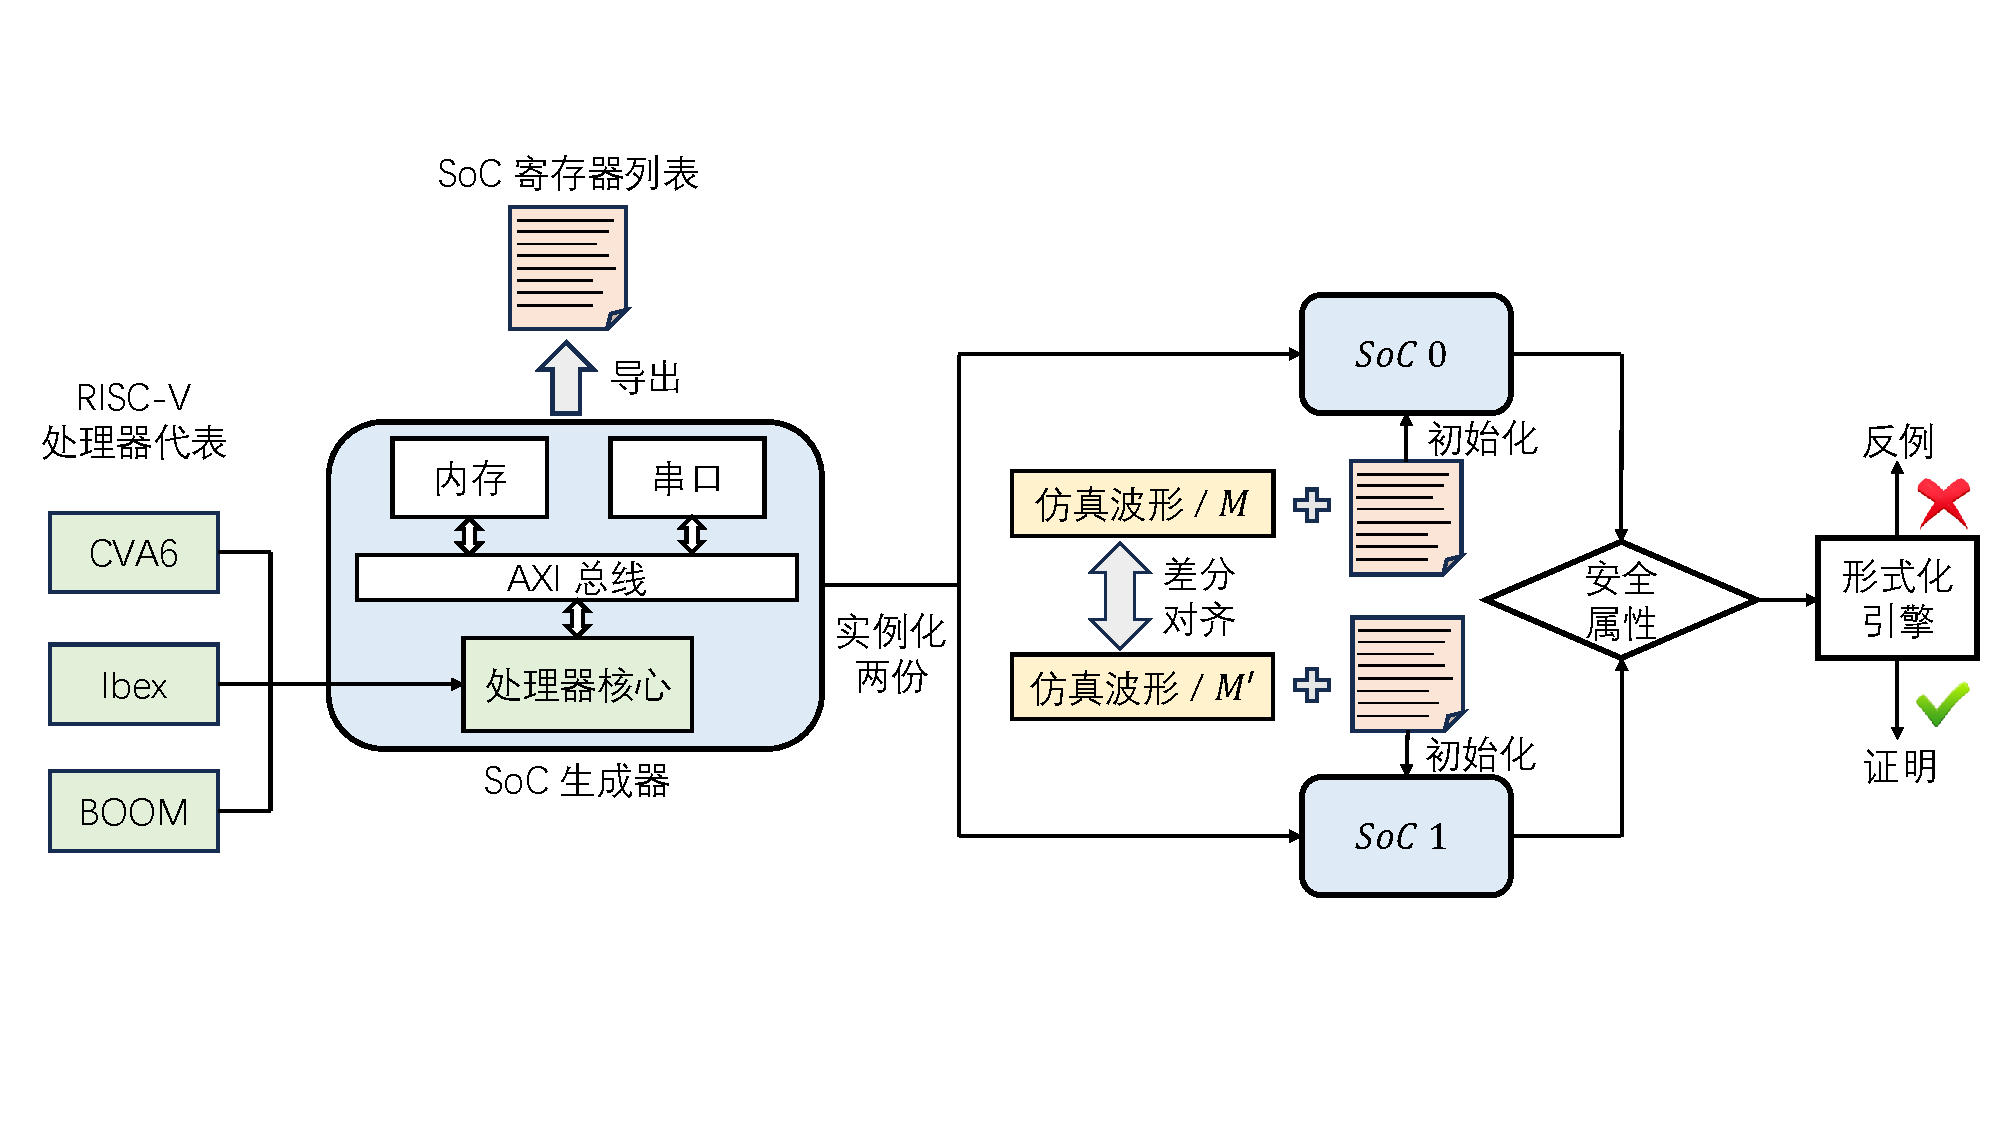
\includegraphics[width=\textwidth]{figure/proposal/Workflow.pdf}
    \caption{RISC-V 处理器侧信道漏洞形式化检测框架工作流程图}
    \label{fig:workflow}
\end{figure}

为了解决以上提出的问题并满足处理器侧信道漏洞检测框架对质量与效率的追求，作者提出了一套新的处理器侧信道漏洞形式化检测框架的流程，试图解决并发展上文所述的三个痛点。
如图 \ref{fig:workflow} 所示，作者首先挑选了几个具有代表性的 RISC-V 处理器核心：
Ibex\cite{ibex}、CVA6\cite{zaruba2019cost} 与 BOOM\cite{zhaosonicboom}， 是当前开源RISC-V生态中最具代表性的三款处理器核心。
然后使用 SoC 生成器\cite{starship}将处理器核心包装到带有总线，内存与串口的 SoC 顶层中。
之后分析 RTL 代码，导出设计中时序单元的变量路径，这个寄存器列表代表着处理器的微架构状态。
同时，将两段只有机密值不同的微架构状态设置程序仿真运行在该 SoC 上，导出两段硬件仿真波形，进行状态对齐。
选择一状态对齐的时钟周期，结合之前导出的寄存器列表，导出寄存器列表当前周期对应的值，并使用该寄存器列表对两个相同的 SoC 进行状态初始化。
最后编写针对两个 SoC 的安全属性，交由形式化引擎对该安全属性进行求解。

针对上文提出的问题和 RISC-V 处理器侧信道漏洞检测框架的工作流程，作者在本节介绍其五个重要的技术路线细节。

\subsubsection{待验证 RISC-V 处理器的选择}
为了评估侧信道漏洞检测框架的通用性，并且增加挖掘漏洞的多样性与影响力，作者决定采用 Ibex\cite{ibex}、CVA6\cite{zaruba2019cost} 与 BOOM\cite{zhaosonicboom} 作为待验证的处理器。
这三款在设计复杂度上覆盖低功耗顺序发射，乱序发射顺序写回，超标量乱序流水线几种架构；
也覆盖了无数据缓存、有缓存且与总线强交互、以及重度推测执行与乱序的完整微架构特征。
同时值得注意的是，Ibex 作为 OpenTitan 信任根项目，在安全性上具有很高的保证；CVA6 和 BOOM 均已流片并在学术界与工业界得到了广泛认可。
如果该漏洞检测框架能够跨越这三种截然不同的微架构稳定发挥作用，将很大程度验证了该框架的有效性与通用性.

\subsubsection{SoC 的构建与时序单元列表的导出}
为了将总线、内存与外设设备纳入验证对象的建模范围中，我们需要通用的 SoC 生成器。
Starship\cite{starship} 能够生成可仿真的 SoC 核外 RTL 代码，并支持方便地替换 SoC 中的处理器核心，也支持将自定义外设设备挂载在总线上。
作者计划引入一个外设设备中常见的 FIFO 外设，如串口，中断控制器等。
这类外设不同于内存，对读操作敏感，可能揭示核内发出的某些未授权的请求，并且普遍存在于真实计算机系统中。

时序单元包括触发器，寄存器与内存单元。
在 SoC 的 RTL 代码中，时序单元本质上是系统状态保持与时序流转的核心载体，是硬件在任意时钟周期下的完整物理快照。
时序单元不仅实例化了指令集可见的架构状态，还隐蔽地包含了了诸如缓存行元数据、分支预测器历史位、推测执行回滚点等海量微架构瞬态信息。
所有时序单元的值的集合决定了 SoC 的状态。作者做出如下定义：
$$state\ =\ flip\ flops\ \cup\ registers\ \cup\ memory\ cells$$
所以作者将对 SoC 中的所有的时序单元进行识别与导出，用作 SoC 状态的记录、分析、导出、同步与恢复。

\subsubsection{微架构状态设置程序的构建与仿真}

为了解决处理器间状态同步的低效率问题和通过形式化符号仿真无法达到处理器深入状态的问题，作者提出了微架构状态设置程序。
在这个程序中，分为本体与变体，即 $M$ 与 $M'$。本体与变体的唯一区别在于 $\texttt{secret}$ 段中一个比特的值不同，除此之外的指令段与数据段完全相同。
这个程序首先会根据建模对象的不同设置好不同的权限，如页表、物理内存保护（PMP）、特权态等。
然后，执行一段随机生成的指令序列；最后会统一跳转到一个固定的地址入口 $\texttt{formal\_entry}$ 处。
将程序本体和程序变体分别编译为二进制文件，送入事先准备好的 SoC 中仿真执行，并导出执行过程中的两段仿真波形轨迹，分别为 $W$ 和 $W'$。

\begin{figure}
    \centering
    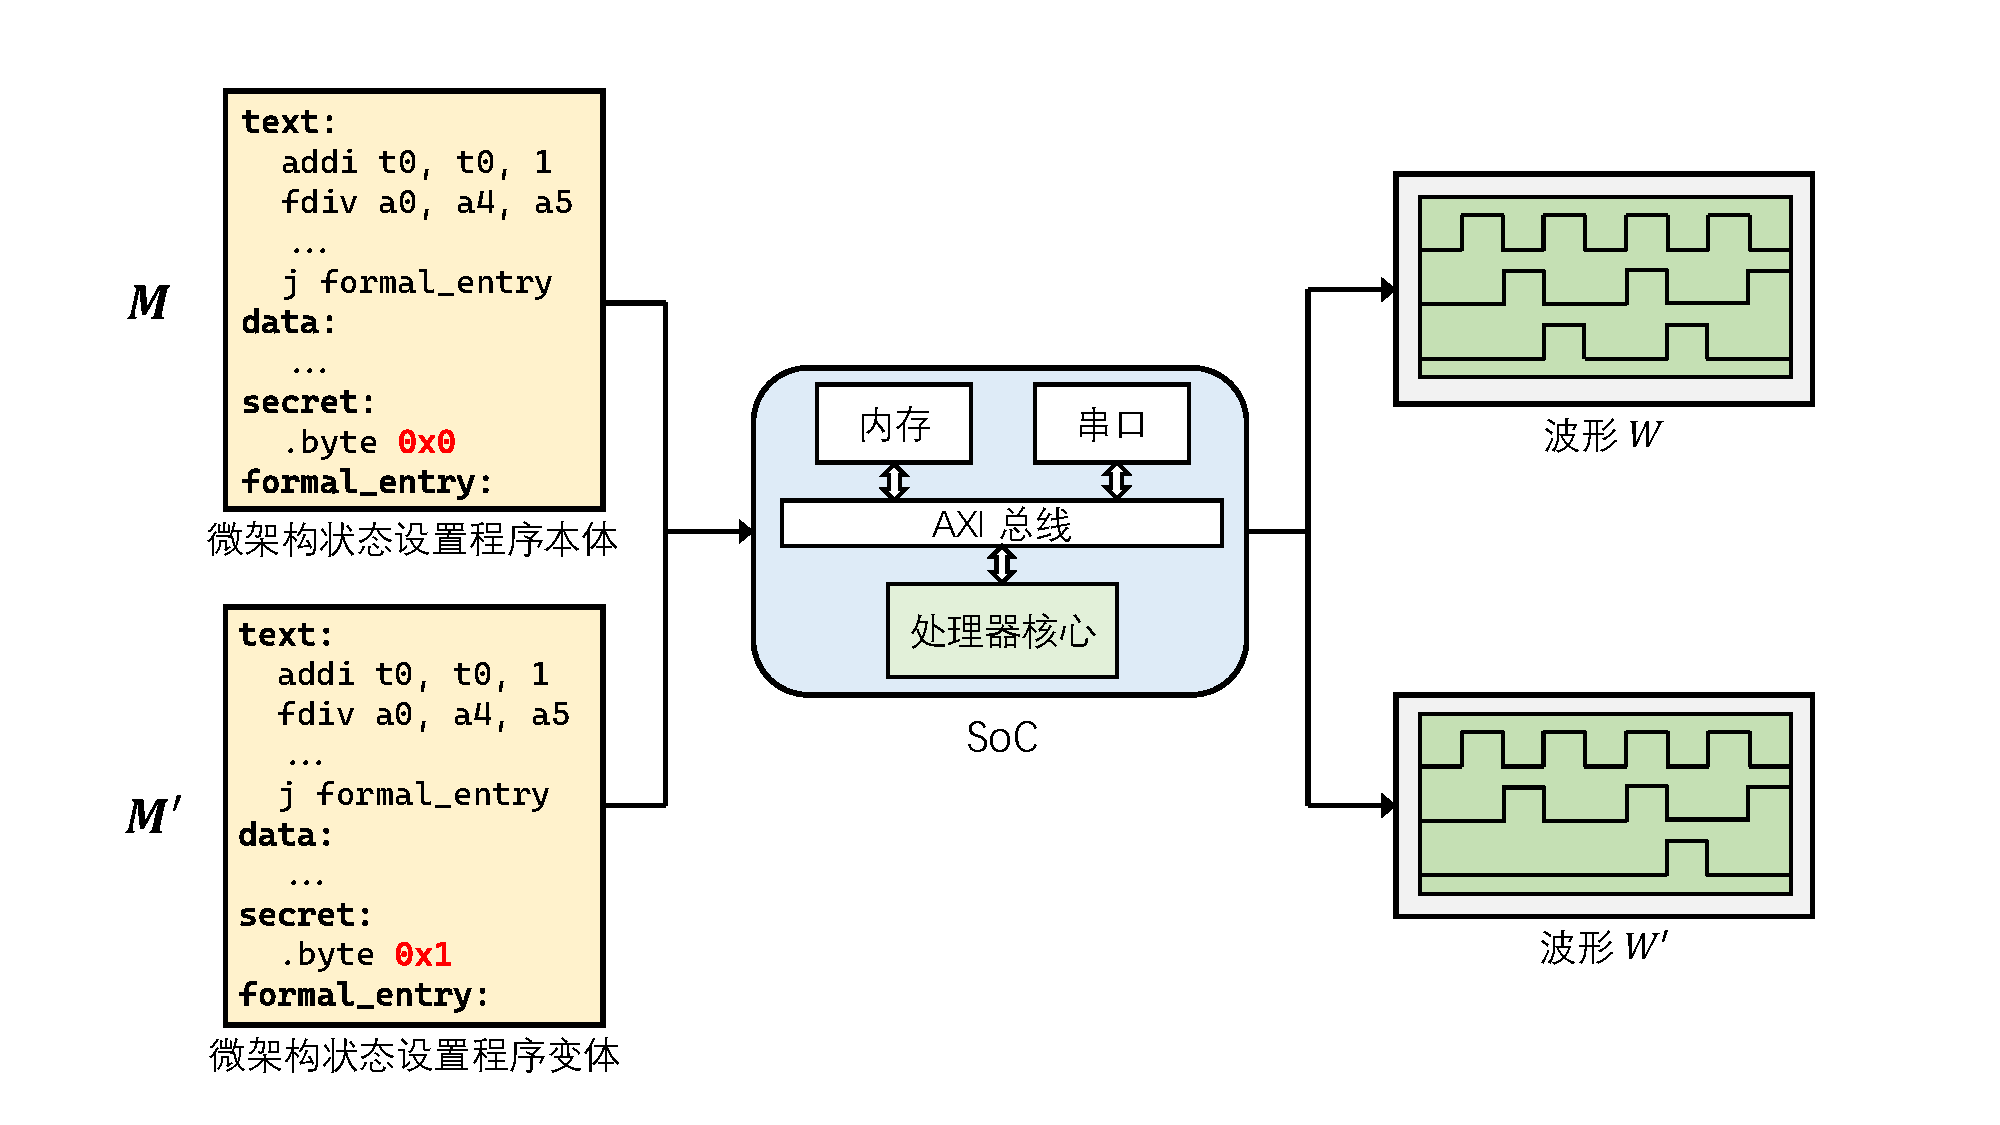
\includegraphics[width=\textwidth]{figure/proposal/variant.pdf}
    \caption{微架构状态设置程序工作流程}
    \label{fig:variant}
\end{figure}

\subsubsection{波形差分对齐与微架构状态初始化}

得到仿真波形 $W$ 和 $W'$ 后，需要对波形进行分析与对齐。
首先，检查两段波形是否出现了分歧，即除了 $secret$ 内存空间外的其他时序单元是否存在差异。
如果不存在差异，则说明之前的微架构状态设置程序还没能够把机密值不同的影响体现到微架构上，需要重新进行微架构设置程序的构建与仿真；
如果存在差异，则说明机密值不同所带来的影响传播到了微架构上，可以进行下一步的差分对齐。

差分对齐指的是找到 $W$ 和 $W'$ 中状态同步的两个时钟周期。
由于机密值的影响，可能导致时序状态产生分歧，如果不进行对齐，则完成微架构状态设置后的两个处理器状态不处于同步状态。
这项工作使用处理器向内存发起对 $\texttt{formal\_entry}$ 地址的取指请求的那个周期作为同步状态的确定周期。
随后将该周期 SoC 时序单元列表中所有项的值从仿真波形 $W$ 和 $W'$ 中导出，得到两个 SoC 在机密值不同的同步状态下的快照。
随后在形式化引擎中使用这两个快照对两个 SoC 进行初始化，这就等价于在形式化求解的开始，处理器就已经到达了一个真实且深入的处理器状态。

\subsubsection{安全属性的设置与形式化求解}

为了覆盖新型的处理器侧信道漏洞，在这项工作中我们引入了新的安全属性，即验证能否通过架构状态来揭示微架构状态。


\subsection{可行性分析}
本项目基于形式化验证中成熟的非干扰理论。
将验证边界从单一的处理器核心拓展至包含总线、内存和外设的 SoC，在理论上消除了由于顶层输入无约束而导致的假阳性问题，满足真实硬件的时序与协议规范。
同时，将微架构状态转化为时序单元的集合，并通过提取同步时钟周期下的硬件快照作为求解的初始状态，这一方法在理论上等价于真实处理器的物理执行快照，保证了形式化验证的可靠性。

本项目选取的验证对象 Ibex、CVA6 与 BOOM 均为当前学术界与工业界广泛认可且高度活跃的开源 RISC-V 处理器项目。
其拥有完整的 RTL 源代码、微架构文档以及配套的编译工具链。
此外，现有的开源 SoC 生成器支持配置处理器核心并挂载 AXI 总线与自定义外设，使得构建符合真实世界约束的 SoC 顶层在技术上可行。

现代成熟的硬件仿真工具如 Verilator， VCS 能够使 SoC 仿真执行 RISC-V 指令，并支持单一时钟周期波形导出。
在状态对齐与初始化阶段，利用 JasperGold 的初始化功能，可以实现硬件的快速状态注入。
同时，现有工作也证明了利用形式化引擎对处理器的安全属性进行求解在时间上是现实的。

传统形式化验证面临的最大问题是状态空间爆炸。本项目提出了先动态仿真预热状态，后静态形式化求解的混合策略。
通过微架构状态设置程序在仿真阶段完成长路径的指令序列执行，仅将状态快照交由形式化引擎进行求解。
这种策略很大地缓解了复杂乱序处理器对求解器造成的计算压力，使得高质量、高效率的侧信道漏洞检测成为可能。